% Et standard slide. Det er vigtigt at [hoved] er inkluderet efter \begin{frame}
\begin{frame}[hoved]
	\frametitle{Introduction}
	\begin{minipage}[t]{0.45\textwidth}
		{\large Context}
		\begin{itemize}
			\item Data centers play an ever increasing role in the IT sector.
			\item Large data movement between CPU and storage plane results in
			      bottleneck for performance.
			\item Computational storage to reduce data movement.
		\end{itemize}
	\end{minipage}
	\hfill
	\begin{minipage}[t]{0.45\textwidth}
		\begin{figure}
			\begin{center}
				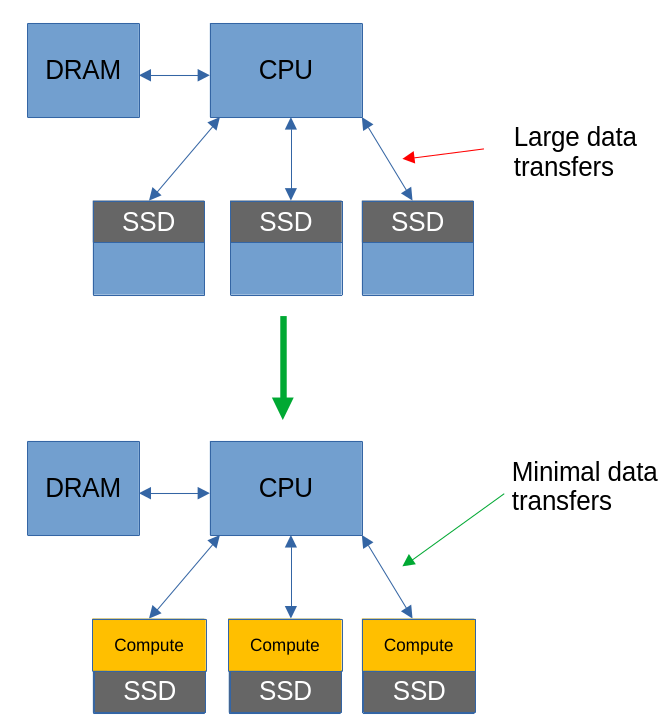
\includegraphics[height=0.55\textheight]{figures/CSD.png}
			\end{center}
			\caption{Traditional architecture vs with CSD.}\label{fig:openssd}
		\end{figure}
	\end{minipage}
\end{frame}

\begin{frame}[hoved]
	\frametitle{Introduction}
	\begin{minipage}[t]{0.45\textwidth}
		{\large Problem and Approach}
		\begin{itemize}
			\item What computation should be handled by a storage device?
			\item Is it feasible to implement such a computation on a RISC-V
			      processor.
			\item Implemented following the RISC-V instruction set architecture.
			\item implemented on the QEMU virtual machine.
		\end{itemize}
	\end{minipage}
	\hfill
	\begin{minipage}[t]{0.45\textwidth}
		\begin{figure}
			\begin{center}
				
\includegraphics[height=0.55\textheight]{figures/qemuvirt.jpeg}
			\end{center}
			\caption{QEMU virtual machine. {\tiny Created using Microsoft
						Designer}}\label{fig:qemu}
		\end{figure}
	\end{minipage}
\end{frame}

